\documentclass[polish,11pt,a4paper]{article}
\usepackage[T1]{fontenc}
\usepackage{graphicx}
\usepackage{amsmath}
\usepackage[polish]{babel}
\usepackage[a4paper, margin=2.5cm]{geometry}
\usepackage{parskip}

\usepackage{amsmath}
\usepackage{graphicx}
\usepackage{float}

%\usepackage{showframe}

\setlength{\parindent}{0pt}

\title{
	{\Huge \textbf{Model Axelroda}}\\
	{\LARGE Badanie wpływu homofilii na trwałość różnorodności kulturowej}
	}
\author{
	Karol Garbaczewski, Szymon Goździkowski, Zofia Sopel, Sasza Tomczyk\\
	Matematyka Stosowana, W13
	}

\begin{document}
	\maketitle
	\section{Wprowadzenie}
	Główny problem przedstawiony w arytkule Roberta Axelroda 
	z 1997 roku pt. „The Dissemination of Culture: 
	A Model with Local Convergence and Global Polarization”
	jest zagadnienie: wiedząc, że wiekszość ludzi upodabnia się do siebie podczas interakcji, 
	to dlaczego cała ludzkość nie stała się jedną monokulturą.
	Axelrod proponuje model oparty na agentach i 
	wielowymiarowych strukturach, twierdząc, że upodobnianie się sąsiadów paradoksalnie 
	prowadzi do trwałego podziału na całkowicie odmienne obozy (globalne polaryzacje).
	Autor proponuję nowatorski model odmmiennych od dotychczasowych, które 
	ograniczają się tylko do jednej poszczególnej cechy.
	\subsection{Tło historyczne}
	W połowie lat 90. XX wieku nastąpił gwałtowny rozwój Internetu, 
	telewizji satelitarnej oraz globalnego handlu.
	Wielu socjologów i politologów wieszczyło szybki
	 koniec różnorodności kulturowej - wchłonięte zostaną lokalne tradycje i obyczaje.
	Jednocześnie równolegle istniały na świecie trwały konflikty
	 o podłożu etnicznym i kulturowym np. wojna w byłej Jugosławii, ludobójstwo w Rwandzie.
	Axelrold wykorzytsał podejście z fizyki statystycznej (modele spinowe), 
	gdzie zderzenie pojedynczych cząstek generuje stan całego układu.


	\section{Założenia modelu}
	 
	Zgodnie z naturalnie dostrzeganą zależnością,
	jesteśmy skłonni wchodzić w interkacje chętniej z osobami podbnymi do nas 
	- komunikacja zachodzi tylko wtedy,
	gdy agenci (jednostki) mają już ze sobą coś wspólnego. 
	Takie zjawisko nazywane jest tytułową homofilia
	 (z języka greckiego - przyjaźń do tego samego).
	\subsection{Konstukcja}
	Axelrod formułuje kulturę jako
	wektor cech np. religia, podobny język, poglądy. Dla każdej cechy istnieje zestaw dopuszczalnych wariantów.
	Dla przykładu 8, 7, 2, 5, 4 oznacza, że kultura zakłada 5 cech, a każda ma 10 wariantów.
	Agenci  rozmieszczeni są na siatce, mogąc wchodzić w interakcje
	wyłącznie ze swoimi bezpośrednimi sąsiadami z prawdopodobieństwem 
	proporcjonalnym do ich obecnego podobieństwa kulturowego, czyli ilości wspólnych cech. 
	Interakcja polega na wylosowaniu cechy, którą się różnią, 
	i zmianie wariantu cechy wybranego agenta na wariant sąsiada, czyli asymilują.

	Gdy dwaj sąsiedzi wchodzą w interakcję, ich podobieństwo rośnie, 
	co zwiększa szansę na kolejne interakcje w przyszłości.
	System osiąga punkt stabilny, gdy każda para sąsiadujących ze 
	sobą jednostek ma kulturowo albo całkowite prawdopodobieństwo,
	czyli kolejne interakcje nic nie zmieniają albo w przeciwnym wypadku interakcje
	 nie są już możliwe. Obserwujemy wtedy powstanie regionów wspólne kulturowo.

	\subsection{Schemat konstrukcji}
	\begin{enumerate}
		\item Losowanie: Program wybiera losowo aktywnego agenta oraz jednego z jego sąsiadów.
		\item Prawdopodobieństwo interakcji: agenci wejdą w interkację w zależności 
		od aktualnego podobieństwa kulturowego (np. dla 3 cech wspolnych na 5 prawdopodobieństwo wynosi 60\%, a gdy brak wspólnych to nie dochodzi do interakcji).
		\item Modyfikacja cechy: agent losowo przyjmuję jedną cechę sąsiada, czyli zwiększa podobieństwo kulturowe.
	\end{enumerate}

	\subsection{Przebieg symulacji}
	\begin{enumerate}
		\item Na początku agenci mają losowo przypisane warianty kulturowe. 
		Większość sąsiadów ma ze sobą bardzo mało wspólnego (dużo różnych kolorów na rys. 1).
		\item W miarę upływu czasu (zdarzeniach) lokalne interakcje powodują, że wspólne warianty kulturowe 
		rozprzestrzeniają się na coraz większe obszary( regiony kulturowe).
		\item Stan stacjonarny: Proces kończy się i stabilizuje, gdy żadna para sąsiadujących jednostek 
		nie może już zmienić swojej kultury (całkowicie identyczni albo całkowicie odmienni).
		\item Wynik końcowy to globalna polaryzacja, czyli kilka całkowicie odizolowanych od siebie, 
		stabilnych regionów kulturowych.  
	\end{enumerate}






	\section{Statystyczne zmiany parametrów}





    \subsection{Model standardowy}
		\begin{figure}[h!]
			\centering
			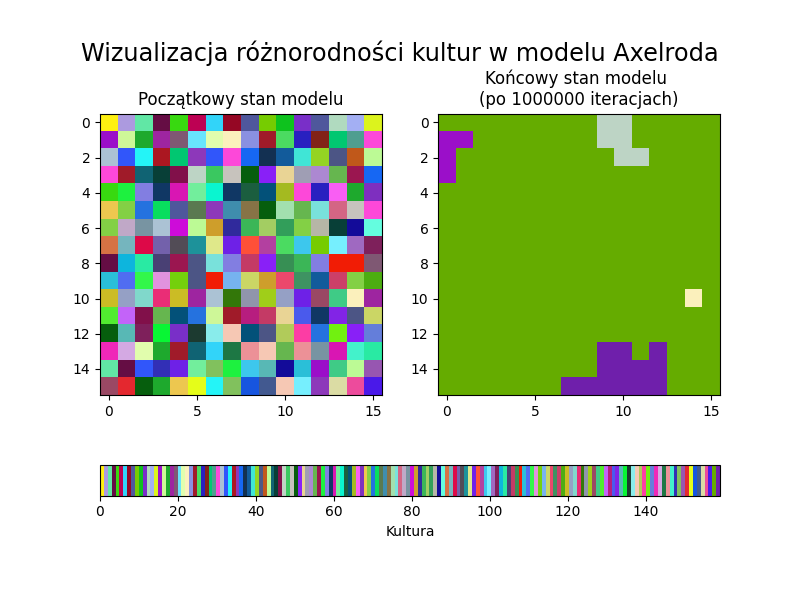
\includegraphics[width=0.8\textwidth]{assets/Grid1.png}
			\caption{Stan stabilny, układ zbiegł do punktów wspólnych kulturowo.}
		\end{figure}




		\begin{figure}[H]
			\centering
			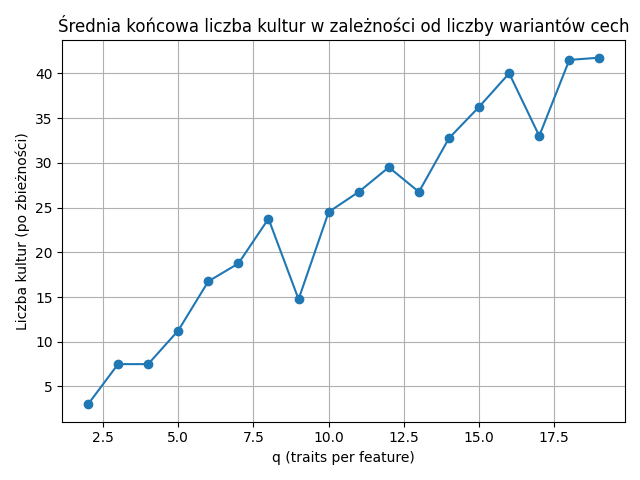
\includegraphics[width=0.8\textwidth]{assets/plot_q_1.png}
			\caption{wiecej wariantow cech wiecej kultur}
			
		\end{figure}


		\begin{figure}[H]
			\centering
			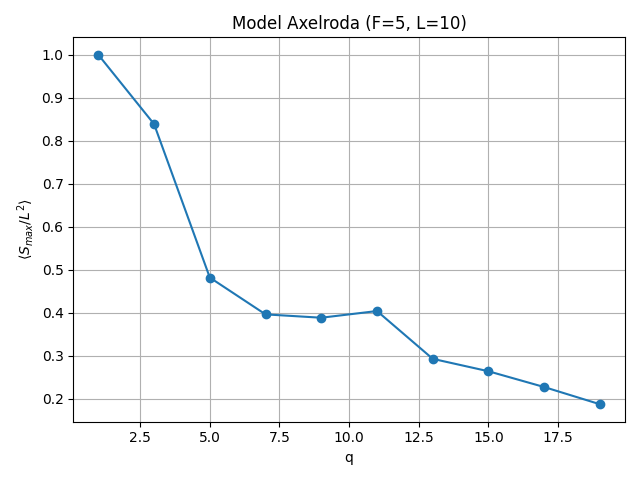
\includegraphics[width=0.8\textwidth]{assets/plot_q_paperlike_1.png}
			\caption{spadkowa im wiecej trade tym mniejszy najwiekszy region}
			
		\end{figure}


		\begin{figure}[H]
			\centering
			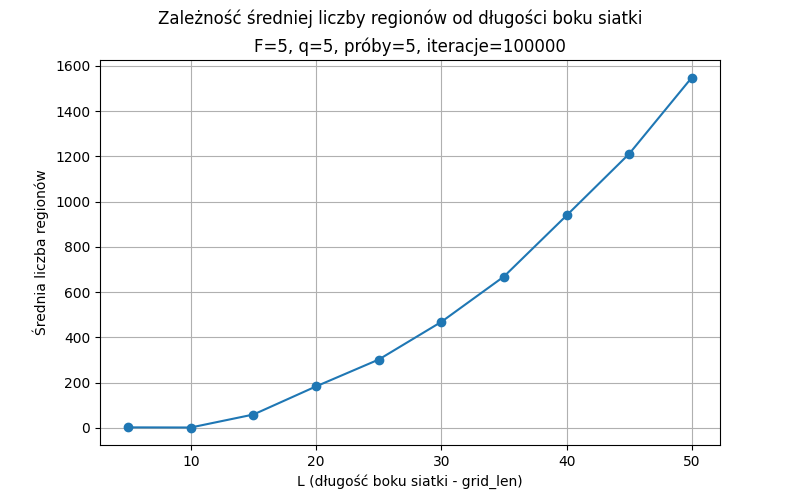
\includegraphics[width=0.8\textwidth]{assets/plot_regions_vs_L_1.png}
			\caption{dluzszy wiecej siatka wiecej regionow}
			
		\end{figure}


		\begin{figure}[H]
			\centering
			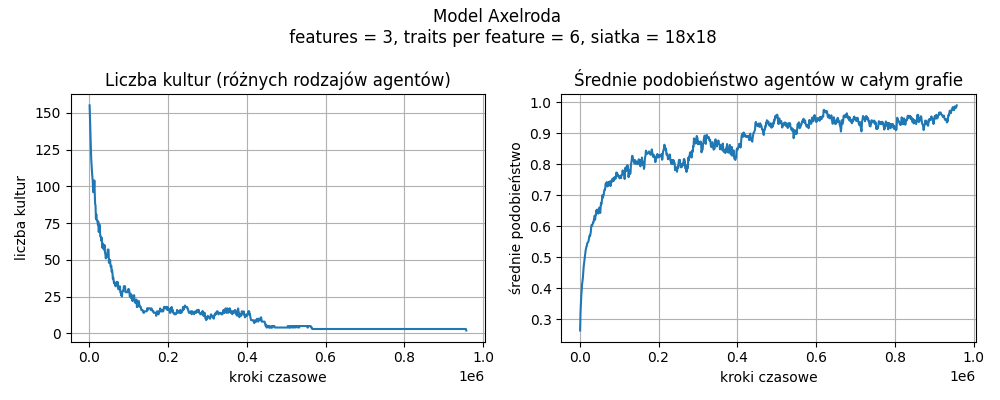
\includegraphics[width=0.8\textwidth]{assets/Plot_t_1.png}
			\caption{wiecej czasu to mniej kultur asymilacja}
			
		\end{figure}
    \subsection{Rozszerzenie modelu}

    Pomysłem na rozwinięcie funkcjonalności modelu jest zmiana sposobu, w jaki członkowie kultur (agenci) są ze sobą połączeni. W standardowym modelu przedstawionym przez Axelroda łączymy agentów na krzyż, tj. agent jest połączony z agentem z lewej, prawej, u góry i na dole. Agenci znajdujący się na brzegu siatki mają natomiast o jednego mniej sąsiada, a Ci w rogach mają w szczególności tylko dwóch.


    W celu zwiększenia przepływu kulturowego ustalamy sąsiedztwo o promieniu 1. To oznacza, że włączamy do sąsiedztwa każdy kierunek, również ukośny. Dla agentów wewnątrz siatki oznacza to 8 agentów sąsiadujących. Sąsiedztwo tworzy wtedy kwadrat \( 3 \times 3\). Nazwiemy ten rodzaj sąsiedztwa \emph{extended}.

    Innym pomysłem jest zadbanie o to, aby agenci na brzegach macierzy nie byli poszkodowani mniejszą liczbą sąsiadów. Dochodzimy do tego poprzez połączenie agenta z jednego brzegu z agentem z brzegu przeciwnego. W praktyce, agent na lewym brzegu jest połączony z agentem tego samego wiersza na prawym brzegu, a np. agent w lewym górnym rogu jest połączony z agentem w prawym dolnym rogu. Sąsiedztwo takie nazwiemy \emph{toroidal}, jako przypominające wzięcie brzegów macierzy i połączenie ich jak torrusa.

    Sprawdziliśmy i porównaliśmy symulacyjnie, jak ma się sprawa zbieżności i liczby regionów dla różnych sąsiedztw.
 1. extended > torroidal > stadard
2. inaczej 
JAKI POWOD SPEKULACJA

		\begin{figure}[H]
			\centering
			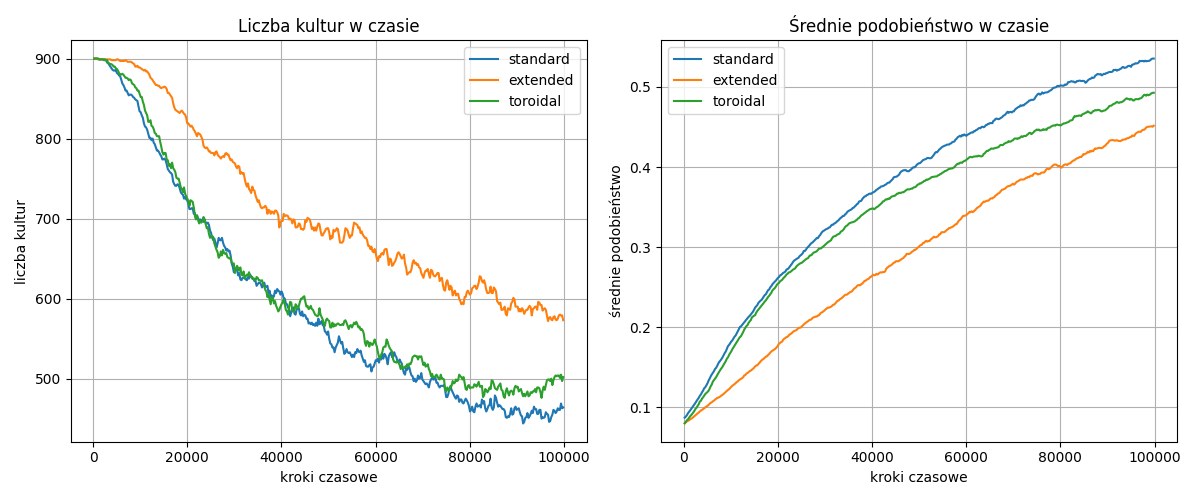
\includegraphics[width=0.8\textwidth]{assets/compare_neighbourhoods_2.png}
			\caption{PIERWSZA SYM}
			
		\end{figure}


		\begin{figure}[H]
			\centering
			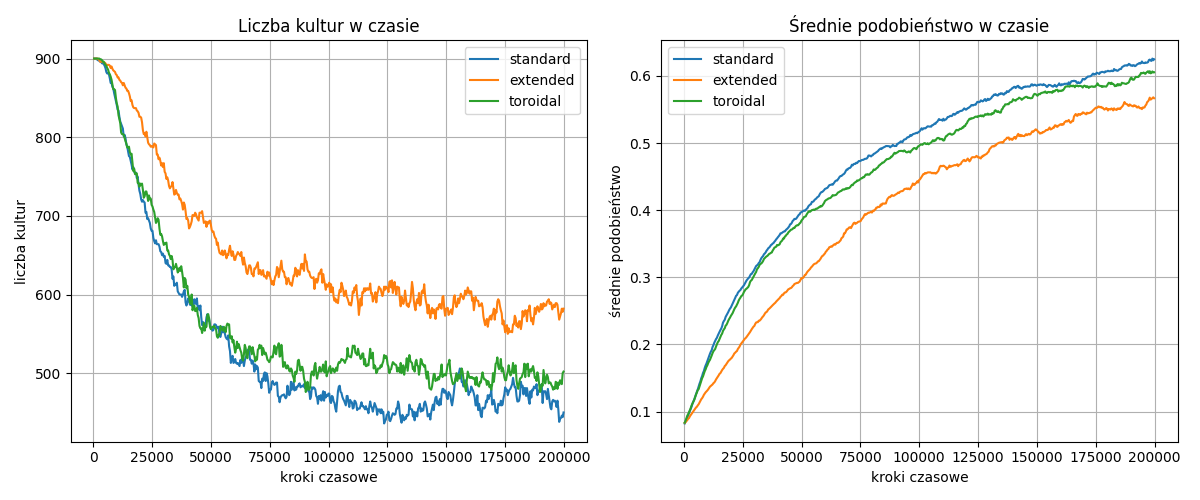
\includegraphics[width=0.8\textwidth]{assets/compare_neighbourhoods_3.png}
			\caption{DRUGA SYM}
			
		\end{figure}



	\section{Wnioski końcowe}

	Najważniejszy wniosek płynący z badań Axelroda wskazuje, że dążenie do lokalnego podobieństwa
	paradoksalnie uniemożliwia całkowite ujednolicenie całego społeczeństwa i utrwala  
	trwałe podziały kulturowe na poziomie globalnym (wyspy wspólne kulturowo).

	Im więcej cech opisuje kulturę, tym mniej stabilnych regionów kulturowych pozostaje na końcu 
	(sprzeczne z intuicją). Dzieje się tak, ponieważ większa liczba cech statystycznie
	 zwiększa szansę posiadania jednego wspólnego elementu, czyli umożliwia interkacje
	  i dalsze zwiększanie wspólnych cech.
	


	%wykresy 
	%modfikacja modelu
	\subsection{Analiza trudności}
	\begin{itemize}
	\item różne metody nie kłóciły się ze sobą i nie psuły nawzajem wyników
	\item przeprowadzanie symulacji nie zmieniało nieodwracalnie badanego układu (można było do niego wrócić)
	\item dobranie czytelnie kolorów
	\item projektowanie obiektowe (klasy)
	\item praca w grupie w szczególności w pisaniu kodu
	\item największą trudnością w implementacji w Pythonie okazała się optymalizacja.

	\end{itemize}	  
	Ogólnie, żeby całość miała ręce i nogi.

	Z łatwych rzeczy fajnie sie implementowało samą podstawę modelu klasy agent i model.
	Bardzo przyjemne szybko można było zacząć bawić się dynamiką modelu nawet bez plotów.
    
    \begin{itemize}

    \item SZYMON CZY ABY NA PEWNO Wyniki symulacji są, w naszej ocenie, naprawdę intuicyjne.
	 Mimo dużej losowości modelu, łatwo przewidzieć jak zmiana parametrów wpływa na szybkość 
	 zbiegania czy liczbę skrystalizowanych regionów kulturowych. Łatwo było również przewidzieć
	  jak rozszerzenie modelu o więcej sąsiadów daje większe możliwości wymiany kulturowej, a 
	  więc szybsze ujednolicenie.


    \end{itemize}


	\section{Zastosowanie w życiu}
	\begin{itemize}
	\item Analiza opinii społecznych (Nature: Ultrametric distribution of culture vectors in 
	an extended Axelrod model of cultural dissemination, Alex Stivala, Garry Robins, Yoshihisa
	 Kashima i Michael Kirley (2014))
	\item Archeologia i antropologia (Toy Story: Homophily, Transmission 
	and the Use of Simple Simulation Models for Assessing Variability in the Archaeological 
	Record, Cornelis J. Drost i Marc Vander Linden (2018))
	\item Badanie mediów społecznościowych i polaryzacji (Cultural Dissemination on Evolving Networks: A Modified Axelrod Model Based on a Rewiring Process, Perez)
	\end{itemize}

	%i te do a-d 
	\section{Podział pracy w grupie}
		\begin{itemize}
			\item Sasza T., Karol G. -> implementacja modelu w języku programowania "Python", programowanie obiektowe agentów, stworzenie funkcji symulacji, tworzenie wykresów w "Matplotlib", aspekt programistyczny  
			
			\item Szymon Gź., Zofia S. ->merytoryczne interpretacja danych z artykułu, symulowanie wyników na podstawie parametrów,
			aspekt humanistyczny przygotowania raportu w \LaTeX
		\end{itemize}

	\section{Bibliografia}
	„The Dissemination of Culture: 
	A Model with Local Convergence and Global Polarization” Roberta Axelrod 97





%########################################################
	%na koniec to usuniemy

dzial???????????????\\
	• Wyniki w formie wykresów (optymalnie dwa): zestawienie wyniku odtworzonego z
	publikacji z nowym wynikiem uzyskanym po modyfikacji modelu.\\
	• Wnioski i przemyślenia:\\


	b) ciekawostki (przede wszystkim zaskakujące zachowania modelu, ale również inne
	nieoczekiwane aspekty realizacji Projektu),\\
	



\end{document}